% Capitulo 3
\chapter{Validation}\label{validationChap}

To validate our guidelines, we searched for open-source tools that could possibly require database transitions. As stated on section \ref{introductionChap}, a database migration is justified when the alternatives have better performance/manutenability than the classic RDBMSs and/or the cost to have a similar performance on the relational database architecture is significantly higher.

This condition (assessing the need for a database transition) is, then, only verifiable on production or simulated environments. Wordpress\cite{wordpress}, world's most popular Content Management System (CMS)  \cite{cmsranking}, can be used to illustrate this problem.  

Wordpress is built on the top of relational databases, such as PostgreSQL and MySQL. So, to justify a database transition on a wordpress-based application, we must \textit{(i)} have access to a deployed and active version of the CMS or \textit{(ii)} build a simulated environment and load it with posts, pages, comments and other entities that are present on a regular wordpress website.

Having access to the production version of a heavily used tool, such as Wordpress, is not easy, as the owner of the CMS must give access to sensible information of its database, users and posts. 

Other open source tools were considered on this phase of the research, such as Redmine \cite{redmine} and Moodle \cite{moodle}, but the same problem that we had trying to accessing sensible information of Wordpress environments was found on these tools.

Besides that, famous open source tools usually have a large user-base. This results in a large support from the community towards the development of the software. With that, if a database transition from RDBMs to NoSQL is needed, it possibly have plugins/addons from the community, as \cite{fantasticElasticsearch}.

Facing this access restrictions to popular open-source projects, to validate the Guidelines proposed on the previous chapter, we have built scenarios that can be easily mapped to real-world applications.

The application proposed on section~\ref{socmediamonitoringapp} is used to illustrate our case studies.

\section{Assessing database transition on a social media monitoring application}
\label{socmediamonitoringapp}

To validate the guidelines presented on Chapter~\ref{theProblemChap} we have modeled \textit{the core database schema} of a social media monitoring  application. Some examples of industry platforms of this kind are \cite{sproutsocial}, \cite{mention} and \cite{buzzmonitor}. 

This category of applications are capable of searching and storing posts from social media platforms, as Twitter and Facebook. On the setup of a new account, users usually define a boolean query of the terms that they want to monitor and the platform starts monitoring \textit{Application Program Interfaces} (APIs) from social networks searching publications that match the boolean query. 

\subsection{Application Requirements and use cases}
\label{appoperations}
From a user perspective, this kind of application might be used to search for relevant topics across social media posts, to be aware of public opinion about brands (brand awareness) or to assess market for a product, for example. 

From a software engineering perspective, some use-cases of this application are:

\begin{enumerate}
\item{\textbf{Create, retrieve, update and delete (CRUD) user account}}
\item{\textbf{CRUD users' terms to monitor}}


\item{\textbf{Retrieve posts by id} - Given a post id, the user is able to visualize it on the interface.}

\item{\textbf{Classify posts (add/tags tags)} - \textit{N} tags (subjects) can be added or removed from a set of posts.}

\item{\textbf{Filter captured posts by filters} - Some possible filters are: 
\begin{itemize}
\item{Boolean Query:} Search posts that mention a boolean query string. \textit{i.e: (Brazil AND Neymar) OR (Orlando AND Kaka)}
\item{Date:} Search posts that were published within a date range. For example: posts from 2015/01/01 to 2015/02/01.
\item{Tags:} Search posts that match a tag query. i.e: posts about ``Soccer Player'' and ``High Salary''.
\end{itemize}
}

\end{enumerate}

Other possible features and use-cases of this kind of applications are not listed to ease the understanding of the scenarios that are presented on the following sections.

\subsection{Application Architecture}
Constuir uma aplicacao desse tipo pode trazer alguns desafios e decisoes a serem feitas. Conforme o escopo da aplicacao cresce, pode ser uma wise decision to quebrar essa grande aplicacao em varias subaplicacoes (ou componentes). 

Alem disso, eh bem custoso que um mesmo source code gerencie tudo da aplicacao, desde a criacao de usuarios ate a coleta e analise automatica de sentimento de posts atraves de processamento de linguagem natural, por exemplo.

Cada um desses componentes pode ter varios outros subcomponentes, ou microservicos. Essa arquitetura de microservicos traz alguns beneficios para a aplicacao, como manutenabilidade, reuso e simplicidade de deploy. Por exemplo, pode ser constuido um microservico que detecte a lingua a partir da string de conteudo de um post e esse microservico poderia ser reaproveitado entre os varios componentes que constituem a aplicacao.   

Arquiteturas baseadas em componentes ou microservicos sao uteis pq permite que utilizemos tecnologias diferentes para servicos diferentes. Assim como no conceito de polyglot persistence, devemos utilizar a melhor tecnologia para cada fim.

Varias subaplicacoes poderiam ser criadas para trabalhar com cada uma das redes sociais suportadas pela aplicacao. Por exemplo: Posso ter uma aplicacao que gerencie e colete todos os conteudos de Facebook, outra que busque os conteudos 
de Twitter, outro de pinterest e etc. 

Na figura X colocamos como seria uma possivel arquitetura baseada em componentes para uma aplicacao Web de monitoramento de redes sociais que monitora o Facebook, Twitter e Google Plus.


\begin{figure}[ht!]
\centering
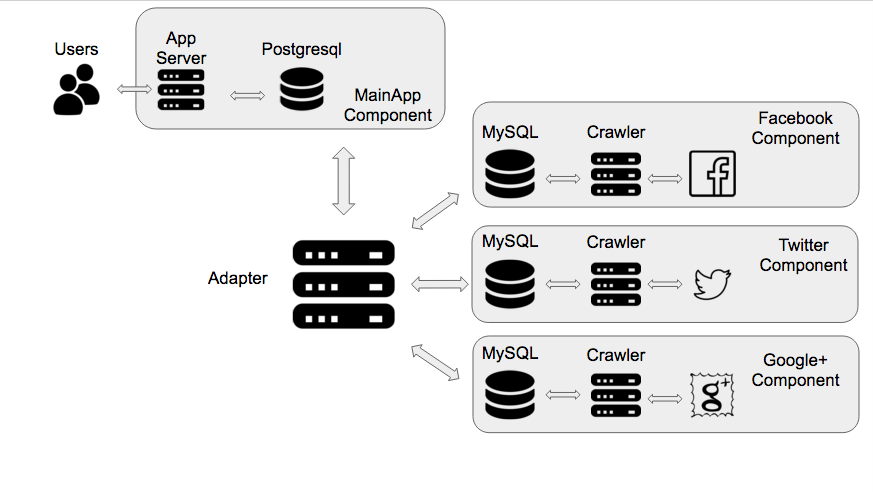
\includegraphics[width=120mm]{Imagens/apparchitecture.png}
\caption{Proposed architecture - Social Media monitoring app.\label{fig:apparchitecture}}
\end{figure}

Na figura e possivel visualizar 5 componentes principais: 

Componente da MainApp: Esse componente pode ser visto como uma aplicacao Web onde o usuario faca login e defina os termos que ele quer monitorar, por exemplo. E nesse componente onde sao feitas todas as edicoes relacionadas aos dados dos usuarios, etc e tal, onde fica a logica de negocio da aplicacao. Esse componente pode ser visto como uma aplicacao de um framework web, como Rails ou Django e e a principal casca da aplicacao. 

Componentes de Facebook, Twitter e Google Plus: Esses componentes sao os responsaveis por interagir com a rede social competente a aquele componente. E interessante que cada rede social tenha seu proprio componente pois e possivel que redes sociais diferentes tenham APIs diferentes, com entidades diferentes e metodos de comunicacao diferentes. Isso eh: o componente de Facebook, por exemplo, pode ter uma API que so se comunica via chamadas HTTP + JSON, o de twitter pode ter uma biblioteca especifica em uma linguagem, ja o de Google Plus pode ter sua comunicacao baseada em SOAP e chamadas via XML, por exemplo. 

Componente Adapter: Esse componente e o responsavel por fazer a integracao entre os diversos bancos de dados que compoem os subsistemas (Facebook, Twitter e Google Plus). 

Como e possivel ver na imagem, ja na etapa de prototipacao dessa aplicacao foi aplicado o conceito de polyglot persistence. No caso dessa aplicacao, dois bancos estao sendo usados: Postgresql e MySQL. Essa decisao pode der sido causada por conta de codigo legado, por exemplo, ou de decisao interna dos arquitetos da aplicacao.



\subsection{Quando a aplicacao cresce, problemas podem aparecer}
\label{shithappens}
Assim que a aplicacao tenha sido lancada, e de se esperar que a performance dela esteja tudo ok. Uma busca de posts no banco de dados da aplicacao, independentemente do numero de filtros, deveria, em tese, retornar em um tempo que seja aceitavel ao usuario. 

Descendo mais um pouco o nivel, e de se esperar que com dezenas ou centenas de posts a aplicacao tenha uma boa performance do ponto de vista do usuario. 
No entanto, pode ser que grandes eventos passem a ser monitorados por essa aplicacao, como a copa do mundo ou as eleicoes de um pais. 

Nesses casos, caso a equipe de engenharia nao tenha feito bons testes de carga da aplicacao, eh bem provavel que a performance da aplicacao e a experiencia do usuario sejam duramente afetadas. Alem disso, conforme o tempo passa, e tambem entendivel que a performance da aplicacao va decaindo, pois aumentarao o numero de posts analisados. 

Dependendo dos termos cadastrados, depois de alguns meses, o numero de posts nas bases MySQL dos tres subsistemas pode crescer bastante, e uma simples consulta que verificava se um post continha uma substring pode passar a analisar milhoes de posts ao inves de centenas. Intuitivamente, como o numero de linhas a serem analisadas aumentara, e de se esperar tambem que o tempo para que essas linhas analisadas tambem aumente. 

\subsection{A aplicacao precisa de outro banco?}
\label{anotherdb}
No cenario descrito, e possivel, por exemplo, que os usuarios da aplicacao passem a reclamar que o tempo de consulta para extrair informacao relevante da plataforma esta altamente insatisfatorio, pois uma consulta que antes era feita em segundos passou a levar minutos ou mesmo horas.

Dado esse cenario de problema, focaremos nossaa analise nos subcomponentes que sao responsaveis pela busca e storage dos posts das redes sociais nos bancos de dados MySQL, mais especificadamente no subcomponente de Facebook. 

A reclamacao de um usuario que uma determinada operacao esta demasiadamente lenta, ou que nao esta no nivel desejado, pode ser causado por uma infinidade de fatores. No cenario descrito na subsecao~\ref{shithappens}, várias coisas podem ter ocorrido: o numero de posts na base pode ter crescido muito e a arquitetura projetada do banco de dados nao esta dando conta, um dos canais de comunicacao entre os servidores do componente Adapter e do Facebook estão falhos, o hardware do fbserver ta muito ruim, etc.

A possible claim from the application users' is that the Search Speed is slowling down as the number of posts grow in the database. In fact, intuition tells us that the search speed slows down as the number of posts in the database grows. 

Relacionados a esse problema, um dos desenvolvedores do componente de facebook pode ter uma forte intuicao de que o problema esta no banco mysql, dizendo que ele nao esta dando mais conta para a quantidade de dados e os requisitos que a aplicacao exige. 

Esse mesmo desenvolvedor pode ainda ter a intuicao de que eh um requisito especifico (uma determinada query SQL) que esta ocasionando essa queda de performance no MySQL, pois essa determinada query pode ficar sendo executada durante um longo tempo, esgotando os recursos de CPU do banco, por exemplo. Intuitivamente, ele pode ainda sugerir que um outro banco NoSQL seria mais apropriado para esse caso de uso.  

Para esse caso, os guidelines propostos na secao anterior casam perfeitamente, pois queremos verificar se existe realmente um problema no MySQL que esta ocasionando essa queda na qualidade do servico oferecido aos usuarios, e se uma transicao a um banco nosql eh mesmo recomendavel ou necessaria. 


\subsection{The application setup: Server}

Nessa subsecao detalhamos um pouco das configuracoes tecnicas dos servidores que foram utilizados para construir parte da aplicacao que apresentamos na secao anterior. 

A cloud server was needed to host the database that is used on the application. We have selected a \textbf{T2.SMALL} instance from \cite{amazonec2} to host it, as it is a general purpose and low-price instance.

T2.SMALL instances feature the following configuration:

\begin{itemize}
\item{High Frequency Intel Xeon Processors with Turbo up to 3.3GHz Burstable CPU, governed by CPU Credits, and consistent baseline performance}
\item{1 vCPU}
\item{12 CPU Credits/hour}
\item{2 GB RAM}
\end{itemize}

\subsection{The application setup: Software}
The machine hosted the following software configuration: 

\begin{itemize}
\item{Operating System: Ubuntu 14.04.2 LTS (GNU/Linux 3.13.0-48-generic x86\_64)}
\item{Secure Shell}
\item{MySQL Version: 14.14 Distrib 5.5.44, for debian-linux-gnu (x86\_64) using readline 6.3}
\end{itemize}

\subsection{The application setup: Data}
To retrieve the data that is used on the scenarios, we have developed a web crawler that gathers posts from Facebook and store them on our MySQL database. 

A total number of 3332534 posts (~ 3 milion posts) were captured and the Dump file with these posts is available on XXXXXXXXXXX. TODO: Upload dump file somewhere. 

\subsection{The application setup: Database schema}
The first database schema was built with the intention of being optimized to production environments, and building \textbf{de}-normalized schemas help to leverage application performance, as revealed by \cite{926306}. 

On Figure~\ref{fig:postsTable} it is possible to view all the columns that compose the \textbf{Posts} table. All post entities, like \textit{message} (content of the post), \textit{link} and \textit{number of likes} are present on this table. 

\begin{figure}[ht!]
\centering
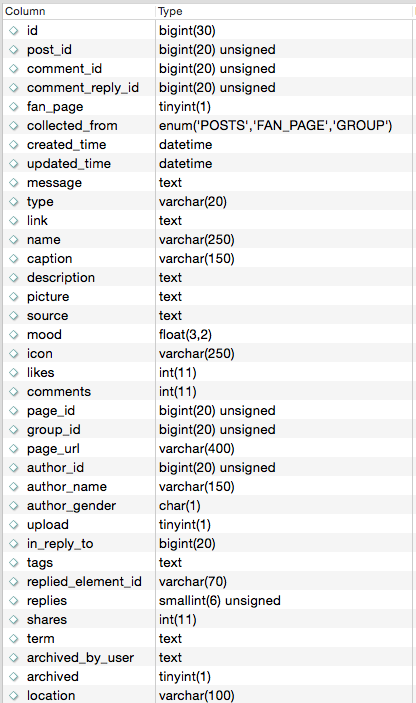
\includegraphics[width=80mm]{postTable.png}
\caption{Posts table.\label{fig:postsTable}}
\end{figure}

Figure~\ref{fig:postsTable} reveals that ``tags'' is a text field on the posts table. Por convencao interna dos desenvolvedores da aplicacao, a tag de um post eh sempre uma mesma substring no formato \textbf{\textit{\#username\_tagname\#}}.

Desse jeito, uma possivel celula de tag poderia ter o seguinte formato: 

\begin{lstlisting}[language=json,firstnumber=1, caption=Tag field standard format, label=tag_field_standard_format]
#username1_tag1##username2_tag1##username3_tag1 
\end{lstlisting}

Se eu quero adicionar uma tag em um post eu simplesmente posso fazer uma concatenacao do post tag com \textbf{\textit{\#username\_tagname\#}}. Da mesma maneira, se eu quero remover essa tag, posso fazer um replace de \textbf{\textit{\#username\_tagname\#}} por uma string vazia.

Essa decisao foi tomada desse jeito para tornar o desenvolvimento da aplicacao mais rapida.


\section{Usando os guidelines}
Como mostrado na secao 3, os guidelines propostos nesse trabalho servem para avaliar e guiar processos de transicoes de bancos de dados em aplicacoes em producao ou em ambientes de simulacao. Podemos usa-los como um bom ponto de partida para avaliar se realmente ha a necessidade de migracao da base ou se o defeito esta em algum outro ponto de falha. 

Ao longo dessa subsecao aplicamos step by step os guidelines mostrados na secao anterior para contextualizar uma transicao de banco de dados na aplicacao apresentada nesta secao. 

Como mostrado previamente \ref{anotherdb}, queremos verificar se ha a necessidade de se trocar o mysql do subcomponente de Facebook da aplicacao proposta em \ref{appoperations} por questao de uma reclamacao do usuario dizendo que uma das operacoes da aplicacao esta com QoS abaixo do esperado.  

\subsection{List application operations that are performed on database-level}
Segundo os guidelines, o primeiro ponto proposto a ser performado num  cenario onde se esta avaliando uma transicao de banco de dados e ``List application enumerations that are performed on database level''. 

No nosso caso, estamos avaliando uma transicao de banco de dados no subsistema de Facebook... Das operacoes citadas na secao \ref{appoperations}, as operacoes que lidam com posts sao apenas \textbf{``Retrieve posts by id''}, \textbf{``Classify posts (add tags)''} and \textbf{``Filter captured posts by filters''}.


\subsection{Define user-centered SLAs}

A secao X revela que para cada uma das operacoes que sao listadas no passo anterior, um conjunto de SLAs deve ser proposto. 

Desse jeito, atraves de conversas com os stakeholders da aplicacao, o seguinte conjunto de SLAs pode ser proposto: 

\textbf{``Retrieve posts by id''}:

Ideal threshold: 3 seconds
Tolerable threshold: 10 seconds
SLA Delta: 10x

\textbf{``Classify posts (add/remove tags)''}:

Ideal threshold: 1.5 second
Tolerable threshold: 3 second
SLA Delta: 3x

\textbf{``Filter captured posts by filters''}:

Ideal threshold: 3 seconds
Tolerable threshold: 10 seconds
SLA Delta: 3.3x


\subsection{Define database-centered SLAs}
Como revelado em secoes anteriores, o usuario e demais stakeholders da aplicacao so sao capazes de identificar SLAs em nivel global, para os casos de uso da aplicacao. No entanto, a equipe de engenharia deve definir tambem SLAs em nivel de bancos de dados. 

Esses SLAs devem ser mais restritivos (apertados) do que os slas definidos pelos usuarios, pois diversas outras acoes tambem sao necessarias para que um caso de uso de um usario seja executado. 

No contexto de uma aplicacao web, por exemplo, sao necessarias verificacoes de tokens de autenticacao, filtragem e conversao de parametros, delays de roteadores e etc.

Desse modo, um conjunto de SLAs de bancos de dados pode ser definido para os 3 use cases propostos: 


\textbf{``Retrieve posts by id''}:

Ideal threshold: 1.0 seconds
Tolerable threshold: 4 seconds
SLA Delta: 4x
ROFR: 30\%

\textbf{``Classify posts (add/remove tags)''}:

Ideal threshold: 0.5 second
Tolerable threshold: 2 second
SLA Delta: 4x

\textbf{``Filter captured posts by filters''}:

Ideal threshold: 2 seconds
Tolerable threshold: 6 seconds
SLA Delta: 3x

\subsection{Build database-level SLA log alerts}

Como a aplicacao proposta nesse trabalho foi idealizada com o proposito de validar esses guidelines, eh possivel afirmar que os log alerts poderiam ser implementados no proprio codigo fonte da aplicacao. Outros servicos, como o New Relic, tambem poderiam ser usados para esse fim, caso a aplicacao ja tivesse uma base de codigo existente. 

Eh indispensavel tambem notar que os verificadores de SLAs so têm utilidade quando existem reqeusts sendo disparadas pelos usuários da aplicacao. Em uma aplicacao hipotetica, essas user requests podem ser simuladas em ferramentas de testes de carga, a exemplo do JMeter, ou ser implementadas como codigo executável.

Em nosso estudo de caso, optamos por construir scripts que simulassem ao mesmo tempo a carga de chamadas dos usuários e que tambem avaliassem se alertas estavam sendo disparados. Atraves desses scripts eh possivel identificar se existe cenarios onde os SLAs propostos na etapa anterior estao sendo quebrados (e consequentemente se ha realmente uma queda na QoS que eh oferecida ao usuario e que eh causada por problemas do lado do banco de dados).

\textbf{Construindo os cenarios de testes}

Foram construidos cenarios de teste para trabalhar com as tres operacoes que foram identificadas na secao \ref{appoperations}. 

Para cada uma dessas situacoes foi implementado um script com checador de quebra de SLA. Ao longo das proximas subsecoes detalhamos como cada script desse foi implementado e discutimos um pouco com relacao aa motivacao da transicao de BD nessa aplicacao de monitoramento de redes sociais.  


\subsubsection{Retrieve posts by id}

O primeiro use-case a ser verificado recuperar um conjunto de posts dado os seus IDs. Essa feature pode ser usada numa listagem de posts, onde pedimos mais detalhes e comentarios sobre um post especifico, por exemplo. Em nivel de banco de dados, essa operacao pode ser enxergada como uma consulta do tipo: 

\begin{lstlisting}[language=json,firstnumber=1, caption=SQL Query - Retrieve posts by ids, label=retrieve_posts_by_ids_sql]
SELECT * FROM posts WHERE id IN (1,2,41,13,12903, ... ,435,31)
\end{lstlisting}\label{query01}

Na etapa anterior, definimos que um SLA a nivel de BD para esse tipo de operacao seria:  

Ideal threshold: 1.0 seconds
Tolerable threshold: 4.0 seconds
SLA Delta: 4x
ROFR: 30\%

Para verificar se essa funcionalidade estava com desempenho abaixo do esperado, foi montado uma rotina de testes de acordo com os seguintes passos: 

\begin{itemize}
\item{Gere uma lista de 100 ids aleatorios que estejam presentes na base de dados.} 
\item{Inicie uma thread que abra uma conexao com o banco de dados e recupere um Result Set com essa lista de posts}
\item{Espere um tempo aleatorio entre 30 e 300 milliseconds (para evitar rajadas de consultas que não ocorreriam em producao) e lance outra thread com o mesmo proposito ate completar um total de 100 threads}
\item{Repita os passos anteriores por 10 vezes}
\end{itemize}

A figura~\ref{fig:core-execution-01} mostra a implementacao desse algoritmo que foi realizada na linguagem Java. \footnote{Essa rotina foi rodada a partir do proprio servidor que hospedava o banco de dados para garantir que o tempo de afericao das queries nao seria afetado por delays causadas na rede interna ou externa.}


\begin{figure}[ht!]
\centering
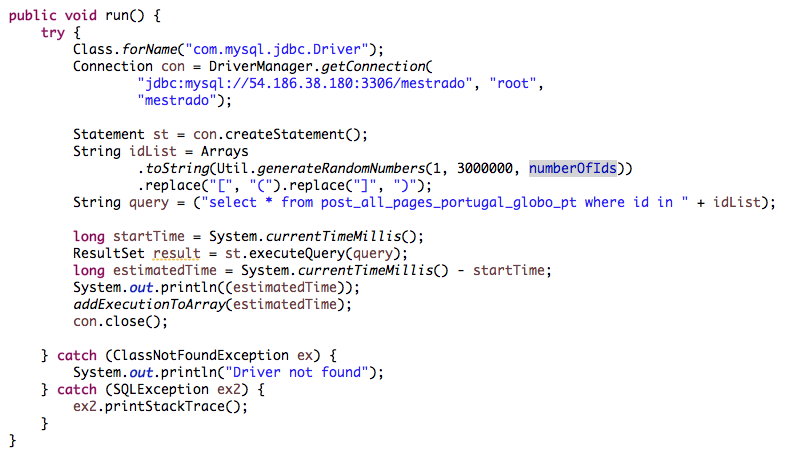
\includegraphics[width=120mm]{Imagens/core-execution-01.png}
\caption{Measurement\label{fig:core-execution-01}}
\end{figure}

A Figura~\ref{fig:first_scenario} mostra o tempo de execucao em milisegundos desse primeiro cenario. No grafico, cada linha representa um experimento de execucao, onde ha repeticoes de 100 vezes de uma consulta no modelo que eh listada no Listing~\ref{retrieve_posts_by_ids_sql}

\begin{figure}[ht!]
\centering
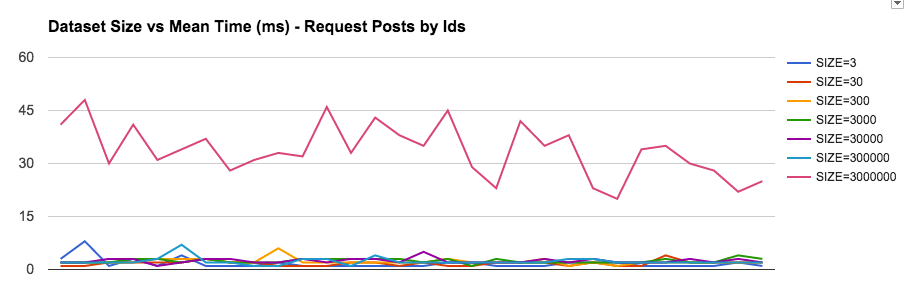
\includegraphics[width=120mm]{Imagens/execution-01.png}
\caption{First Scenario - Retrieve post by ids.\label{fig:first_scenario}}
\end{figure}


Como o ideal threshold para esse requisito states that as consultas sejam executadas em ate 1000 milisegundos (um segundo), podemos afirmar que o MySQL seria mais que suficiente para garantir a execucao desse requisito. Eh importante ressaltar que nas 1.000 consultas do experimento, nenhuma query rompeu a barreira do ideal threshold. 

Eh facil perceber que para esse requisito o MySQL nao eh de maneira alguma um gargalo, pois todas as consultas estao sendo retornadas em um tempo inferior a 40 milisegundos. 

A Figura \ref{fig:sla_check} mostra a implementacao Java de uma thread que faz as requisicoes ao MySQL e as coloca em um arraylist que eh usado para fins de logging.

\begin{figure}[ht!]
\centering
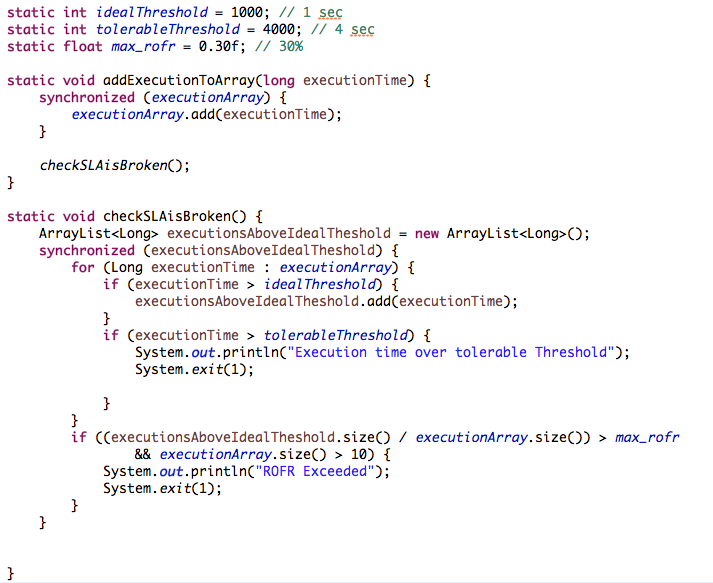
\includegraphics[width=120mm]{Imagens/check_sla.png}
\caption{Check SLA Violation.\label{fig:sla_check}}
\end{figure}

No Apendice~\ref{executionreport02} eh possivel visualizar os dados crus desse grafico. 

\subsubsection{Classify posts (add/remove tags) - Not Ready}


\subsubsection{Filter captured posts by filters - Not Ready}

To verify this scenario within our database, we have implemented a runnable SLA checker in Python programming language. The algorithm, shown on Figure~\ref{fig:algorithmSLA01} performs fulltext-search operations on our MySQL database and verifies if the SLA is broken in this scenario. 

First, we define several query sizes, and for each query size we generate random strings. Then, a query with of the following style is performed on our MySQL Database: 

 ``SELECT COUNT(*) FROM posts WHERE message like \%myQueryString\%''

For each query size, we repeat the operation with a distinct word for three times (NUMBER\_OF\_ATTEMPTS\_FOR\_EACH\_QUERY\_LENGTH = 3). On our experiments, we found out that there's no noticeable difference between querying random generated ascii-chars and words from the dictionary.

\begin{figure}[ht!]
\centering
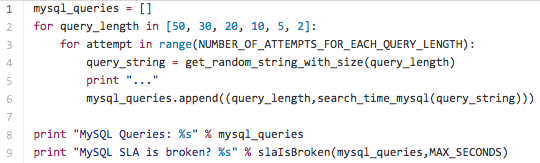
\includegraphics[width=100mm]{algorithmSLA01.png}
\caption{Runnable SLA v0.1 .\label{fig:algorithmSLA01}}
\end{figure}	

We have tested the scenario with [100, 1000,10000, 100000, 100000, 1000000, 2000000 and 30000] posts within our dataset. Execution reports shows us that, indeed, the first SLO is broken with a data-size of 1000000 (one million) posts.

Execution reports for each of these dataset values is available on Appendix B.

% \subsection{Guidelines}
% % % The \textbf{first step} of our guidelines states that to propose a database migration, it is necessary to identify that a requirement of the application is broken. In this case, the search speed requirement is broken).

% % % The \textbf{second step} is to implement a runnable SLA that shows that the Service Level Objective is not being fulfilled. The runnable SLA that was explained shows that the Search Operation Time SLO is not being met. 

% % \textbf{Step number three} is to show that the requirement (or SLO) is broken. Execution Report 01, available on Appendix~\ref{executionreport01} shows that Steps 1, 2 and 3 of our guidelines are done. 

% \textbf{The fourth step} of the guidelines is to propose modifications on the relational database. 

% TODO finish here. http://blog.scoutapp.com/articles/2014/12/19/from-mysql-full-text-search-to-elasticsearch reporta algumas opcoes para melhorar a performance de um full text search com MySQL. 

Dentre as opcoes para melhorar o processo de search, ele aponta duas solucoes: (i) ``To support full-text search, we needed to use the MySQL MyISAM storage engine. This has major downsides, the primary one being full table locks: when a table is updated, no other changes to that table can be performed.'' A outra saida era (ii) ``We ended up doing this. It was a fairly simple step and allowed us to switch to the InnoDB engine on the master, eliminating the table lock issues.

This bought us some time, but it wasn't a long-term solution: we basically were rolling our own search and this frequently involved complex queries that third-party search libraries could perform more efficiently. We ended up with massive queries composed of many JOINs plus AND/ORs - these aren't easy to maintain.

Besides query complexity, it's tough to beat the performance of a dedicated search solution. Our tables have considerable update activity, so this would result in sometimes-significant performance issues.
''
Outros contra-pontos para implementar fulltext search em MySQL apontado por XXX, XXX and XXX sao X Y e Z. Falta terminar essa parte.

\subsection{Verify SLA violation - Not ready}

Para resolver o problema apontado no passo anterior, movemos a estrutura das tags para uma tabela separada. 

On Figure~\ref{fig:tagTable} it is possible to verify the elements that compose a \textbf{Tag} record. Each tag has a unique ID - \textit{idtags}, a \textit{post\_id} (foreign key to the post table), a \textit{tag\_user} (the username of the user who has tagged this post) and \textit{tag\_name}, the subject of this post. 

The Tags table is also denormalized, as \textit{tag\_user} and \textit{tag\_name} are entities that should be represented on separate tables on a normalized schema.

\begin{figure}[ht!]
\centering
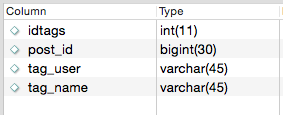
\includegraphics[width=60mm]{tagTable.png}
\caption{Tags table.\label{fig:tagTable}}
\end{figure}

\textbf{Tags} information is purposely redundant. This way, it is possible to retrieve the tags of a post from a \textbf{JOIN} query between the Tags and Post tables and by searching it within the \textit{tags} column of the Posts table. This data-redundancy was planned to test which option has better performance on a production scenario.  


\subsection{Propose architectural changes at database-level - Not ready}

Apache Solr, Lucene, Amazon Cloudsearch and Elasticsearch are \textbf{Search Engines} that provide fulltext-search as master-features. 

Elasticsearch (a.k.a. Elastic) was seemed to be a good alternative to the problem that we were facing with MySQL. Some discussion forums were consulted and comparisons and studies were considered on our research \cite{StackOverflowElastic} \cite{SolrVsES} \cite{quoraES}. With that, \textbf{step number four} is done. 

A new data model should be proposed once the new database technology is chosen. As Elasticsearch stores data as JSON documents, the same structure of post that we had on the posts table was transformed into a valid JSON document.

A new server with the same configuration of the one presented on the beginning of this chapter was provisioned and Elasticsearch[1.7.2] version was installed.

To dump the data from MySQL and import to Elasticsearch, a Python script was made \cite{mysqltoes}. However, loading data was taking too long as the script didn't paralellize the bulk insert queries on Elasticsearch and database connection kept dropping. To overcome this situation,an open-source project that connects to MySQL via JDBC and imports data into Elasticsearch \cite{elasticjdbc} was used. 
With that, \textbf{the sixth step} is successfully executed. 

A new runnable SLA was necessary to compare the execution time of the previous database architecture (MySQL) and the one that was proposed. We have joined both runnable SLAs into a single script, available on \cite{runnablesla01}, \textbf{finishing the seventh step}.

It is possible to compare the Execution Report of both database architectures on Execution Report 02 (Appendix \ref{executionreport01}).

With that, it is possible to show that the runnable SLA on the new architecture with all posts results in a significant performance improvement, proving that a database transition may be suitable to this scenario, \textbf{finishing Step 08}.


\subsection{Map current schema \& data on the proposed DB architecture}

\subsection{Process all DB operations from a historical point}


% To proceed with a DB migration, Scenarios 02 and 03 must also be analyzed. 

% \abrv[UFRN -- Universidade Federal do Rio Grande do Norte]{UFRN}

% \section{Scenario 03}
% Update by query Scenario. 

% Elasticsearch doesn't support natively. 

% Update by query plugin

% MySQL wins

% Dizer tambem que o pessoal recomenda migrar pedacos de feature a feature, como nesse case do Coursera. https://tech.coursera.org/blog/2014/09/23/courseras-adoption-of-cassandra/
